
% LaTeX Beamer file automatically generated from DocOnce
% https://github.com/hplgit/doconce

%-------------------- begin beamer-specific preamble ----------------------

\documentclass{beamer}

\usetheme{metropolis}
\usecolortheme{default}

% turn off the almost invisible, yet disturbing, navigation symbols:
\setbeamertemplate{navigation symbols}{}

% Exemples on customization:
%\usecolortheme[named=RawSienna]{structure}
%\usetheme[height=7mm]{Rochester}
%\setbeamerfont{frametitle}{family=\rmfamily,shape=\itshape}
%\setbeamertemplate{items}[ball]
%\setbeamertemplate{blocks}[rounded][shadow=true]
%\useoutertheme{infolines}
%
%\usefonttheme{}
%\useinntertheme{}
%
%\setbeameroption{show notes}
%\setbeameroption{show notes on second screen=right}

% fine for B/W printing:
%\usecolortheme{seahorse}

\usepackage{pgf}
\usepackage{graphicx}
\usepackage{epsfig}
\usepackage{relsize}

\usepackage{fancybox}  % make sure fancybox is loaded before fancyvrb

\usepackage{fancyvrb}
\usepackage{minted} % requires pygments and latex -shell-escape filename
%\usepackage{anslistings}
%\usepackage{listingsutf8}

\usepackage{amsmath,amssymb,bm}
%\usepackage[latin1]{inputenc}
\usepackage[T1]{fontenc}
\usepackage[utf8]{inputenc}
\usepackage{colortbl}
\usepackage[english]{babel}
\usepackage{tikz}
\usepackage{framed}
% Use some nice templates
\beamertemplatetransparentcovereddynamic

% --- begin table of contents based on sections ---
% Delete this, if you do not want the table of contents to pop up at
% the beginning of each section:
% (Only section headings can enter the table of contents in Beamer
% slides generated from DocOnce source, while subsections are used
% for the title in ordinary slides.)
\AtBeginSection[]
{
  \begin{frame}<beamer>[plain]
  \frametitle{}
  %\frametitle{Outline}
  \tableofcontents[currentsection]
  \end{frame}
}
% --- end table of contents based on sections ---

% If you wish to uncover everything in a step-wise fashion, uncomment
% the following command:

%\beamerdefaultoverlayspecification{<+->}

\newcommand{\shortinlinecomment}[3]{\note{\textbf{#1}: #2}}
\newcommand{\longinlinecomment}[3]{\shortinlinecomment{#1}{#2}{#3}}

\definecolor{linkcolor}{rgb}{0,0,0.4}
\hypersetup{
    colorlinks=true,
    linkcolor=linkcolor,
    urlcolor=linkcolor,
    pdfmenubar=true,
    pdftoolbar=true,
    bookmarksdepth=3
    }
\setlength{\parskip}{7pt}  % {1em}

\newenvironment{doconceexercise}{}{}
\newcounter{doconceexercisecounter}
\newenvironment{doconce:movie}{}{}
\newcounter{doconce:movie:counter}

\newcommand{\subex}[1]{\noindent\textbf{#1}}  % for subexercises: a), b), etc

\logo{{\tiny \copyright\ 2023, UP Mathématiques. ESPRIT}}

%-------------------- end beamer-specific preamble ----------------------

% Add user's preamble




% insert custom LaTeX commands...

\raggedbottom
\makeindex

%-------------------- end preamble ----------------------

\begin{document}

% matching end for #ifdef PREAMBLE

\newcommand{\exercisesection}[1]{\subsection*{#1}}



% ------------------- main content ----------------------



% ----------------- title -------------------------

\title{Introduction à Python}

% ----------------- author(s) -------------------------

\author{UP Mathématiques\inst{1}}
\institute{École Supérieure PRivée d'Ingénierie et de Technologies (ESPRIT).\inst{1}}
% ----------------- end author(s) -------------------------

\date{2 novembre 2023
\\ \ \\ 
\centerline{
\includegraphics[width=0.45\linewidth]{imgs/Signature-01.jpg}}
\ \\ 
{\tiny \copyright\ 2023, UP Mathématiques. ESPRIT}
}

\vspace{6mm}



\vspace{6mm}

\begin{frame}[plain,fragile]
\titlepage
\end{frame}

\section{Objectifs généraux en premier}

\begin{frame}[plain,fragile]
\frametitle{Objectifs généraux en premier}


Une partie essentielle de ce cours est de vous permettre de faire de la science par des expériences numériques et de développer des projets qui vous permettent d'étudier des systèmes complexes. Le but est d'améliorer ce que nous appelons la pensée algorithmique.

\noindent\textbf{Algorithme}
Un ensemble fini d'instructions non ambiguës qui, étant donné un ensemble de conditions initiales, peuvent être effectuées dans une séquence prescrite pour atteindre un certain but.


\end{frame}

\section{Situation standard que nous rencontrons quotidiennement}

\begin{frame}[plain,fragile]
\frametitle{Situation standard que nous rencontrons quotidiennement}


La situation standard que nous rencontrons presque tous les séances de cours:

\begin{itemize}
\item Théorie + expérience + simulation est presque la norme dans la recherche et l'industrie.

\item Être capable de modéliser des systèmes complexes. Résoudre de vrais problèmes.

\item Accent la compréhension des principes fondamentaux et des lois dans les sciences.

\item Être capable de visualiser, présenter, discuter, interpréter et venir avec une analyse critique des résultats, et développer une attitude éthique saine pour son propre travail.

\item Améliorer le raisonnement sur la méthode scientifique.
\end{itemize}

\noindent
Une bonne présentation des résultats obtenus via de bons rapports scientifiques, aide à inclure tous les aspects ci-dessus.


\end{frame}

\section{Langage Python}

\begin{frame}[plain,fragile]
\frametitle{Langage Python}


\href{{http://www.python.org/}}{Python} est un langage de programmation moderne de haut niveau, orienté objet et d'usage général.

\textbf{Caractéristiques générales de Python} :

\begin{itemize}
\item Langage simple:
\begin{itemize}

  \item facile à lire et à apprendre avec une syntaxe minimaliste.

\end{itemize}

\noindent
\item Langage concis et expressif:
\begin{itemize}

  \item moins de lignes de code

  \item moins de bugs

  \item plus facile à maintenir.
\end{itemize}

\noindent
\end{itemize}

\noindent

\end{frame}

\begin{frame}[plain,fragile]
% No title on this slide

\textbf{Détails techniques} :

\begin{itemize}
\item Typé dynamiquement:
\begin{itemize}

  \item Pas besoin de définir le type des variables, les arguments ou le type des fonctions.

\end{itemize}

\noindent
\item La gestion automatique de la mémoire:
\begin{itemize}

  \item Aucune nécessité d'allouer explicitement et désallouer la mémoire pour les variables et les tableaux de données. Aucun bug de fuite de mémoire.

\end{itemize}

\noindent
\item Interprété:
\begin{itemize}

  \item Pas besoin de compiler le code. L'interpréteur Python lit et exécute le code python directement.
\end{itemize}

\noindent
\end{itemize}

\noindent
\end{frame}

\begin{frame}[plain,fragile]
% No title on this slide

\textbf{Avantages} :

\begin{itemize}
\item Le principal avantage est la facilité de programmation, qui minimise le temps nécessaire pour développer, déboguer et maintenir le code.

\item Langage bien conçu qui encourage les bonnes pratiques de programmation:
\begin{itemize}

  \item Modulaire et orientée objet, permet l'encapsulation  et la réutilisation de code. Il en résulte souvent un code plus transparent, plus facile à améliorer et sans bug.

  \item Documentation intégré avec le code.

\end{itemize}

\noindent
\item De nombreuses bibliothèques standards, et de nombreux packages add-on.
\end{itemize}

\noindent
\end{frame}

\section{Installation d'un environnement Python scientifique}

\begin{frame}[plain,fragile]
\frametitle{Installation d'un environnement Python scientifique}




\noindent\textbf{Qu’est ce que Anaconda ?}
L’installation d’un environnement Python complet peut-être une vraie galère. Déjà, il faut télécharger Python et l’installer. Par la suite, télécharger un à un les packages dont on a besoin. Parfois, le nombre de ces librairies peut-être grand.

Par ailleurs, il faut s’assurer de la compatibilité entre les versions des différentes packages qu’on a à télécharger. Bref, ce n’est pas amusant.


\end{frame}

\begin{frame}[plain,fragile]
% No title on this slide

\href{{https://www.anaconda.com/download/}}{Anaconda} est  une distribution Python. A son installation, Anaconda installera Python ainsi qu'une multitude de packages (voir \href{{https://docs.anaconda.com/anaconda/packages/pkg-docs#python-3-6}}{liste de packages anaconda}).  Cela nous évite de nous ruer dans les problèmes d’incompatibilités entre les différents packages.

Finalement, Anaconda propose un outil de gestion de packages appelé \href{{https://conda.io/docs/}}{conda}. Ce dernier permettra de mettre à jour et installer facilement les librairies dont on aura besoin pour nos développements.
\end{frame}

\begin{frame}[plain,fragile]
% No title on this slide

\noindent\textbf{Préparer la formation: téléchargement d’Anaconda.}
Nous demandons à tous les étudiants de télécharger Anaconda. Pour cela, il faut télécharger un installeur à partir de \href{{https://www.anaconda.com/download/}}{\nolinkurl{https://www.anaconda.com/download/}}, correspondant à votre système d’exploitation (Windows, Mac OS X, Linux). Il faut choisir entre 32 bits ou 64 bits (pour la version \emph{Python 3}) selon que votre système d’exploitation est 32 bits ou 64 bits.
\end{frame}

\begin{frame}[plain,fragile]
% No title on this slide

\begin{figure}[!ht]  % 
  \centerline{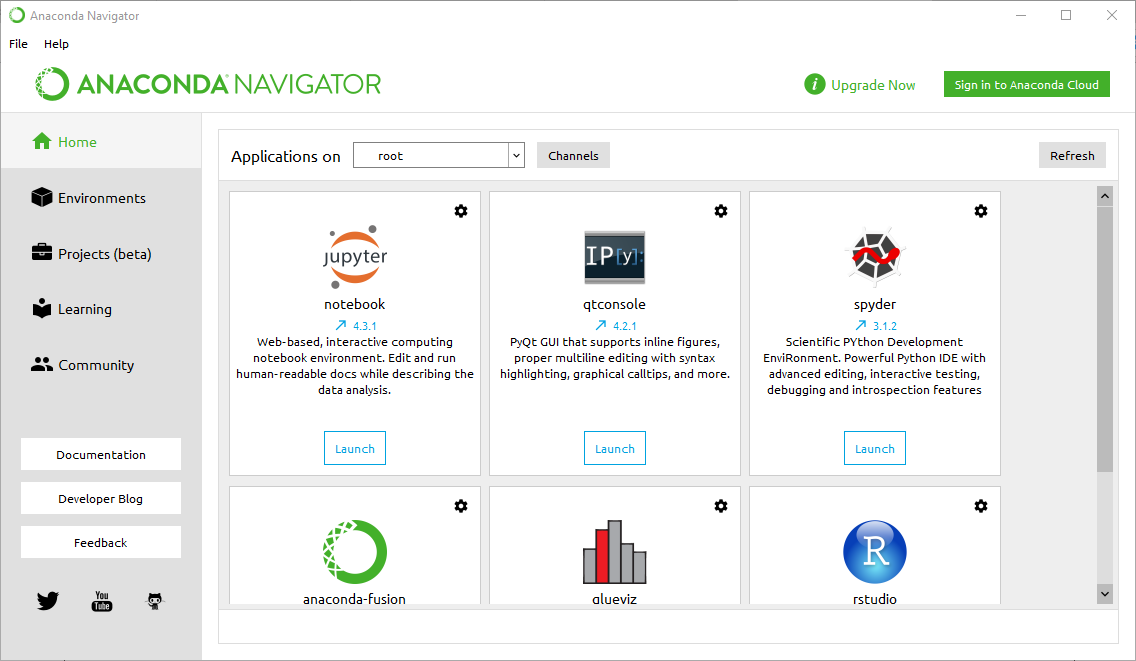
\includegraphics[width=0.7\linewidth]{imgs/AnacondaNavigator.png}}
  \caption{
  Interface graphique du navigateur Anaconda sur Windows
  }
\end{figure}
%\clearpage % flush figures
\end{frame}

\begin{frame}[plain,fragile]
% No title on this slide

\begin{block}{Note}
Anaconda installe plusieurs exécutables pour développer en Python dans le répertoire \emph{anaconda/bin}, sans toujours créer des raccourcis sur le bureau ou dans un menu. Nous nous occuperons au tout début de la formation de créer des raccourcis pour pouvoir lancer l'application web \emph{Jupyter notebook}. Vous pouvez lancer le notebook depuis le navigateur Anaconda.
\end{block}
\end{frame}

\section{Introduction: "Hello World!"}

\begin{frame}[plain,fragile]
\frametitle{Introduction: "Hello World!"}

C'est devenu une tradition que lorsque vous apprenez un nouveau langage de programmation, vous démarrez avec un programme permettant à l'ordinateur d'imprimer le message \emph{"Hello World!"}.

\begin{minted}[fontsize=\fontsize{9pt}{9pt},linenos=false,mathescape,baselinestretch=1.0,fontfamily=tt,xleftmargin=2mm]{python}
In [1]: print("Hello World!")
Hello World!
\end{minted}

Félicitation! tout à l'heure vous avez fait votre ordinateur saluer le monde en anglais! La fonction \texttt{print()} est utilisée pour imprimer l’instruction entre les parenthèses. De plus, l'utilisation de guillemets simples \Verb?print('Hello World!')? affichera le même résultat. Le délimiteur de début et de fin doit être le même.

\begin{minted}[fontsize=\fontsize{9pt}{9pt},linenos=false,mathescape,baselinestretch=1.0,fontfamily=tt,xleftmargin=2mm]{python}
In [2]: print('Hello World!')
Hello World!
\end{minted}


\end{frame}

\section{Commentaires}

\begin{frame}[plain,fragile]
\frametitle{Commentaires}


Au fur et à mesure que vos programmes deviennent plus grands et plus compliqués, ils deviennent plus difficiles à lire et à regarder un morceau de code et à comprendre ce qu'il fait ou pourquoi. Pour cette raison, il est conseillé d’ajouter des notes à vos programmes pour expliquer en langage naturel ce qu’il fait. Ces notes s'appellent des commentaires et commencent par le symbole \Verb!#!.

Voyez ce qui se passe lorsque nous ajoutons un commentaire au code précédent:

\begin{minted}[fontsize=\fontsize{9pt}{9pt},linenos=false,mathescape,baselinestretch=1.0,fontfamily=tt,xleftmargin=2mm]{python}
In [3]: print('Hello World!') # Ceci est mon premier commentaire
Hello World!
\end{minted}
Rien ne change dans la sortie? Oui, et c’est très normal, l’interprète Python ignore cette ligne et ne renvoie rien. La raison en est que les commentaires sont écrits pour les humains, pour comprendre leurs codes, et non pour les machines.


\end{frame}

\section{Nombres}

\begin{frame}[plain,fragile]
\frametitle{Nombres}


L'interpréteur Python agit comme une simple calculatrice: vous pouvez y taper une expression et l'interpréteur restituera la valeur. La syntaxe d'expression est simple: les opérateurs +, -, * et / fonctionnent comme dans la plupart des autres langages (par exemple, Pascal ou C); les parenthèses (\texttt{()}) peuvent être utilisées pour le regroupement. Par exemple:

\begin{minted}[fontsize=\fontsize{9pt}{9pt},linenos=false,mathescape,baselinestretch=1.0,fontfamily=tt,xleftmargin=2mm]{python}
In [4]: 5+3
Out[4]: 8
In [5]: 2 - 9      # les espaces sont optionnels
Out[5]: -7
In [6]: 7 + 3 * 4  #la hiérarchie des opérations mathématique
Out[6]: 19
In [7]: (7 + 3) * 4  # est-elle respectées?
Out[7]: 40
# en python3 la division retourne toujours un nombre en virgule flottante
In [8]: 20 / 3
Out[8]: 6.666666666666667
In [9]: 7 // 2      # une division entière
Out[9]: 3
\end{minted}


\end{frame}

\begin{frame}[plain,fragile]
% No title on this slide

On peut noter l’existence de l’opérateur \Verb!%! (appelé opérateur modulo). Cet opérateur fournit le reste de la division entière d’un nombre par un autre. Par exemple :

\begin{minted}[fontsize=\fontsize{9pt}{9pt},linenos=false,mathescape,baselinestretch=1.0,fontfamily=tt,xleftmargin=2mm]{python}
In [10]: 7 % 2       # donne le reste de la division
Out[10]: 1
In [11]: 6 % 2
Out[11]: 0
\end{minted}

Les exposants peuvent être calculés à l'aide de doubles astérisques \texttt{**}.

\begin{minted}[fontsize=\fontsize{9pt}{9pt},linenos=false,mathescape,baselinestretch=1.0,fontfamily=tt,xleftmargin=2mm]{python}
In [12]: 3**2
Out[12]: 9
\end{minted}

Les puissances de dix peuvent être calculées comme suit:

\begin{minted}[fontsize=\fontsize{9pt}{9pt},linenos=false,mathescape,baselinestretch=1.0,fontfamily=tt,xleftmargin=2mm]{python}
In [13]: 3 * 2e3   # vaut 3 * 2000
Out[13]: 6000.0
\end{minted}
\end{frame}

\section{Affectations (ou assignation)}

\begin{frame}[plain,fragile]
\frametitle{Affectations (ou assignation)}



Dans presque tous les programmes Python que vous allez écrire, vous aurez des variables. Les variables agissent comme des espaces réservés pour les données. Ils peuvent aider à court terme, ainsi qu’à la logique, les variables pouvant changer, d’où leur nom. C’est beaucoup plus facile en Python car aucune déclaration de variables n’est requise. Les noms de variable (ou tout autre objet Python tel que fonction, classe, module, etc.) commencent par une lettre majuscule ou minuscule (A-Z ou a-z). Ils sont sensibles à la casse (\texttt{VAR1} et \texttt{var1} sont deux variables distinctes). Depuis Python, vous pouvez utiliser n’importe quel caractère Unicode, il est préférable d’ignorer les caractères ASCII (donc pas de caractères accentués).

Si une variable est nécessaire, pensez à un nom et commencez à l'utiliser comme une variable, comme dans l'exemple ci-dessous:


\end{frame}

\begin{frame}[plain,fragile]
% No title on this slide

Pour calculer l'aire d'un rectangle par exemple: \texttt{largeur} x \texttt{hauteur}:

\begin{minted}[fontsize=\fontsize{9pt}{9pt},linenos=false,mathescape,baselinestretch=1.0,fontfamily=tt,xleftmargin=2mm]{python}
In [15]: largeur = 25
In [16]: hauteur = 40
In [17]: largeur    # essayer d'accéder à la valeur de la variable largeur
Out[17]: 25
\end{minted}

on peut également utiliser la fonction \texttt{print()} pour afficher la valeur de la variable \texttt{largeur}

\begin{minted}[fontsize=\fontsize{9pt}{9pt},linenos=false,mathescape,baselinestretch=1.0,fontfamily=tt,xleftmargin=2mm]{python}
In [16]: print(largeur)
25
\end{minted}
Le produit de ces deux variables donne l'aire du rectangle:
\begin{minted}[fontsize=\fontsize{9pt}{9pt},linenos=false,mathescape,baselinestretch=1.0,fontfamily=tt,xleftmargin=2mm]{python}
In [17]: largeur * hauteur  # donne l'aire du rectangle
Out[17]: 1000
\end{minted}
\end{frame}

\begin{frame}[plain,fragile]
% No title on this slide

\begin{block}{Note}
Notez ici que le signe égal (\texttt{=}) dans l'affectation ne doit pas être considéré comme \textbf{"est égal à"}. Il doit être \textbf{"lu"} ou interprété comme \textbf{"est définie par"}, ce qui signifie dans notre exemple:

\begin{quote}
La variable \texttt{largeur} est définie par la valeur 25 et la variable \texttt{hauteur} est définie par la valeur 40.
\end{quote}

\end{block}

\begin{block}{Avertissement}
Si une variable n'est pas \emph{définie} (assignée à une valeur), son utilisation vous donnera une erreur:

\begin{minted}[fontsize=\fontsize{9pt}{9pt},linenos=false,mathescape,baselinestretch=1.0,fontfamily=tt,xleftmargin=2mm]{python}
In [18]: aire     # essayer d'accéder à une variable non définie
-----------------------------------------------------------------------
NameError                            Traceback (most recent call last)
<ipython-input-18-1b03529c1ce5> in <module>()
----> 1 aire     # essayer d'accéder à une variable non définie

NameError: name 'aire' is not defined
\end{minted}
\end{block}
\end{frame}

\begin{frame}[plain,fragile]
\frametitle{Noms de variables réservés (keywords)}

Laissez-nous résoudre ce problème informatique (ou \textbf{bug} tout simplement)!. En d'autres termes, assignons la variable \texttt{aire} à sa valeur.

\begin{minted}[fontsize=\fontsize{9pt}{9pt},linenos=false,mathescape,baselinestretch=1.0,fontfamily=tt,xleftmargin=2mm]{python}
In [19]: aire = largeur * hauteur
In [20]: aire  # et voila!
Out[20]: 1000
\end{minted}


Certains noms de variables ne sont pas disponibles, ils sont réservés à python lui-même. Les mots-clés suivants (que vous pouvez afficher dans l'interpréteur avec la commande \texttt{help("keywords")}) sont réservés et ne peuvent pas être utilisés pour définir vos propres identifiants (variables, noms de fonctions, classes, etc.).
\end{frame}

\begin{frame}[plain,fragile]
% No title on this slide

\begin{minted}[fontsize=\fontsize{9pt}{9pt},linenos=false,mathescape,baselinestretch=1.0,fontfamily=tt,xleftmargin=2mm]{python}
In [20]: help("keywords")

Here is a list of the Python keywords.  Enter any keyword to get more help.

False               def                 if                  raise
None                del                 import              return
True                elif                in                  try
and                 else                is                  while
as                  except              lambda              with
assert              finally             nonlocal            yield
break               for                 not
class               from                or
continue            global              pass

# par exemple pour éviter d'écraser le nom réservé lambda
In [22]: Lambda = 630e-9
In [23]: Lambda
Out[23]: 6.3e-07
\end{minted}
\end{frame}

\begin{frame}[plain,fragile]
\frametitle{Les types}

Les types utilisés dans Python sont: integers, long integers, floats (double prec.), complexes, strings, booleans. La fonction \texttt{type()} donne le type de son argument
\noindent\textbf{Le type int (integer : nombres entiers).}
Pour affecter (on peut dire aussi assigner) la valeur 20 à la variable nommée \texttt{age} :

\begin{minted}[fontsize=\fontsize{9pt}{9pt},linenos=false,mathescape,baselinestretch=1.0,fontfamily=tt,xleftmargin=2mm]{python}
age = 20
\end{minted}
La fonction \texttt{print()} affiche la valeur de la variable :

\begin{minted}[fontsize=\fontsize{9pt}{9pt},linenos=false,mathescape,baselinestretch=1.0,fontfamily=tt,xleftmargin=2mm]{python}
In [24]: print(age)
20
\end{minted}
La fonction \texttt{type()} retourne le type de la variable :
\begin{minted}[fontsize=\fontsize{9pt}{9pt},linenos=false,mathescape,baselinestretch=1.0,fontfamily=tt,xleftmargin=2mm]{python}
type(age)
Out[25]: int
\end{minted}
\end{frame}

\begin{frame}[plain,fragile]
% No title on this slide

\noindent\textbf{Le type float (nombres en virgule flottante).}
\begin{minted}[fontsize=\fontsize{9pt}{9pt},linenos=false,mathescape,baselinestretch=1.0,fontfamily=tt,xleftmargin=2mm]{python}
b = 17.0  # le séparateur décimal est un point (et non une virgule)
b
Out[26]: 17.0
In [27]: type(b)
Out[27]: float
In [28]: c = 14.0/3.0
    ...: c
Out[28]: 4.666666666666667
\end{minted}
Notation scientifique :
\begin{minted}[fontsize=\fontsize{9pt}{9pt},linenos=false,mathescape,baselinestretch=1.0,fontfamily=tt,xleftmargin=2mm]{python}
In [29]: a = -1.784892e4
    ...: a
Out[29]: -17848.92
\end{minted}
\end{frame}

\begin{frame}[plain,fragile]
% No title on this slide

\noindent\textbf{Les fonctions mathématiques.}
Pour utiliser les fonctions mathématiques, il faut commencer par importer le module \texttt{math} :

\begin{minted}[fontsize=\fontsize{9pt}{9pt},linenos=false,mathescape,baselinestretch=1.0,fontfamily=tt,xleftmargin=2mm]{python}
import math
\end{minted}
La fonction \texttt{help()} retourne la liste des fonctions et données d'un module.

Soit par exemple: \texttt{help('math')}
\end{frame}

\begin{frame}[plain,fragile]
% No title on this slide

Pour appeler une fonction d'un module, la syntaxe est la suivante : \texttt{module.fonction(arguments)}

Pour accéder à une donnée d'un module : \texttt{module.data}

\begin{minted}[fontsize=\fontsize{9pt}{9pt},linenos=false,mathescape,baselinestretch=1.0,fontfamily=tt,xleftmargin=2mm]{python}
 # donnée pi du module math (nombre pi)
In [32]: math.pi
Out[32]: 3.141592653589793
# fonction sin() du module math (sinus)
In [33]: math.sin(math.pi/4.0)
Out[33]: 0.7071067811865475
# fonction sqrt() du module math (racine carrée)
In [34]: math.sqrt(2.0)
Out[34]: 1.4142135623730951
# fonction exp() du module math (exponentielle)
In [35]: math.exp(-3.0)
Out[35]: 0.049787068367863944
# fonction log() du module math (logarithme népérien)
In [36]: math.log(math.e)
Out[36]: 1.0
\end{minted}
\end{frame}

\begin{frame}[plain,fragile]
% No title on this slide

\noindent\textbf{Le type complexe.}
Python possède par défaut un type pour manipuler les nombres complexes. La partie imaginaire est indiquée grâce à la lettre « \texttt{j} » ou « \texttt{J} ». La lettre mathématique utilisée habituellement, le « \texttt{i} », n’est pas utilisée en Python car la variable i est souvent utilisée dans les boucles.

\begin{minted}[fontsize=\fontsize{9pt}{9pt},linenos=false,mathescape,baselinestretch=1.0,fontfamily=tt,xleftmargin=2mm]{python}
In [37]: a = 2 + 3j
    ...: type(a)
Out[37]: complex
In [38]: a
Out[38]: (2+3j)
\end{minted}
\end{frame}

\begin{frame}[plain,fragile]
% No title on this slide

\begin{block}{Avertissement}
\begin{minted}[fontsize=\fontsize{9pt}{9pt},linenos=false,mathescape,baselinestretch=1.0,fontfamily=tt,xleftmargin=2mm]{python}
In [39]: b = 1 + j
--------------------------------------------------------------
NameError                      Traceback (most recent call last)
<ipython-input-39-0f22d953f29e> in <module>()
----> 1 b = 1 + j

NameError: name 'j' is not defined
\end{minted}
Dans ce cas, on doit écrire la variable \texttt{b} comme suit:
\begin{minted}[fontsize=\fontsize{9pt}{9pt},linenos=false,mathescape,baselinestretch=1.0,fontfamily=tt,xleftmargin=2mm]{python}
In [41]: b = 1 + 1j
    ...: b
Out[41]: (1+1j)
\end{minted}
sinon Python va considérer \texttt{j} comme variable non définie.
\end{block}
\end{frame}

\begin{frame}[plain,fragile]
% No title on this slide

\noindent\textbf{Le type str (string : chaîne de caractères).}
\begin{minted}[fontsize=\fontsize{9pt}{9pt},linenos=false,mathescape,baselinestretch=1.0,fontfamily=tt,xleftmargin=2mm]{python}

In [43]: nom = 'Tounsi' # entre apostrophes
    ...: nom
Out[43]: 'Tounsi'
In [44]: type(nom)
Out[44]: str
In [45]: prenom = "Ali"  # on peut aussi utiliser les guillemets
    ...: prenom
Out[45]: 'Ali'
In [46]: print(nom, prenom)  # ne pas oublier la virgule
Tounsi Ali
\end{minted}
\end{frame}

\begin{frame}[plain,fragile]
% No title on this slide

La concaténation désigne la mise bout à bout de plusieurs chaînes de caractères.
La concaténation utilise l'opérateur \texttt{+}:
\begin{minted}[fontsize=\fontsize{9pt}{9pt},linenos=false,mathescape,baselinestretch=1.0,fontfamily=tt,xleftmargin=2mm]{python}
In [47]: chaine = nom + prenom  # concaténation de deux chaînes de caractères
    ...: chaine
Out[47]: 'TounsiAli'
\end{minted}
Vous voyez dans cet exemple que le nom et le prénom sont collé. Pour ajouter une espace entre ces deux chaînes de caractères:
\begin{minted}[fontsize=\fontsize{9pt}{9pt},linenos=false,mathescape,baselinestretch=1.0,fontfamily=tt,xleftmargin=2mm]{python}
In [48]: chaine = prenom + ' ' + nom
    ...: chaine # et voila
Out[48]: 'Ali Tounsi'
\end{minted}
\end{frame}

\begin{frame}[plain,fragile]
% No title on this slide

On peut modifier/ajouter une nouvelle chaîne à notre variable \texttt{chaine} par:
\begin{minted}[fontsize=\fontsize{9pt}{9pt},linenos=false,mathescape,baselinestretch=1.0,fontfamily=tt,xleftmargin=2mm]{python}
In [49]: chaine = chaine + ' 22 ans'  # en plus court : chaine += ' 22 ans'
    ...: chaine
Out[49]: 'Ali Tounsi 22 ans'
\end{minted}

La fonction \texttt{len()} renvoie la longueur (\emph{length}) de la chaîne de caractères :

\begin{minted}[fontsize=\fontsize{9pt}{9pt},linenos=false,mathescape,baselinestretch=1.0,fontfamily=tt,xleftmargin=2mm]{python}
In [53]: print(nom)
    ...: len(nom)
Tounsi
Out[53]: 6
\end{minted}
\end{frame}

\begin{frame}[plain,fragile]
% No title on this slide

\noindent\textbf{Indexage et slicing :}

\begin{Verbatim}[numbers=none,fontsize=\fontsize{9pt}{9pt},baselinestretch=0.95]
 +---+---+---+---+---+---+
|------------------------|
 | T | o | u | n | s | i |
 +---+---+---+---+---+---+
 |------------------------|
 0   1   2   3   4   5   6
 --->
-6  -5  -4  -3  -2  -1
                   <----
\end{Verbatim}
\begin{minted}[fontsize=\fontsize{9pt}{9pt},linenos=false,mathescape,baselinestretch=1.0,fontfamily=tt,xleftmargin=2mm]{python}
In [55]: nom[0]  # premier caractère (indice 0)
Out[55]: 'T'

In [56]: nom[:] # toute la chaine
Out[56]: 'Tounsi'

In [57]: nom[1] # deuxième caractère (indice 1)
Out[57]: 'o'
\end{minted}
\end{frame}

\begin{frame}[plain,fragile]
% No title on this slide

\begin{minted}[fontsize=\fontsize{9pt}{9pt},linenos=false,mathescape,baselinestretch=1.0,fontfamily=tt,xleftmargin=2mm]{python}
In [58]: nom[1:4]   # slicing
Out[58]: 'oun'

In [59]: nom[2:]  # slicing
Out[59]: 'unsi'

In [60]: nom[-1]   # dernier caractère (indice -1)
Out[60]: 'i'

In [61]: nom[-3:]    # slicing
Out[61]: 'nsi'

\end{minted}
\end{frame}

\begin{frame}[plain,fragile]
% No title on this slide

\begin{block}{Avertissement}

On ne peut pas mélanger le type \texttt{str} et type \texttt{int}.

Soit par exemple:
\begin{minted}[fontsize=\fontsize{9pt}{9pt},linenos=false,mathescape,baselinestretch=1.0,fontfamily=tt,xleftmargin=2mm]{python}
In [63]: chaine = '22'
    ...: annee_naissance = 2018 - chaine
----------------------------------------------------------
TypeError                  Traceback (most recent call last)
<ipython-input-63-8607078f78d2> in <module>()
      1 chaine = '22'
----> 2 annee_naissance = 2018 - chaine

TypeError: unsupported operand type(s) for -: 'int' and 'str'
\end{minted}
\end{block}
\end{frame}

\begin{frame}[plain,fragile]
% No title on this slide

Pour corriger cette erreur, la fonction \texttt{int()} permet de convertir un type \texttt{str} en type \texttt{int}:

\begin{minted}[fontsize=\fontsize{9pt}{9pt},linenos=false,mathescape,baselinestretch=1.0,fontfamily=tt,xleftmargin=2mm]{python}

In [64]: nombre = int(chaine)
In [65]: type(nombre) # et voila!
Out[65]: int
\end{minted}

Maintenant on peut trouver \Verb!annee_naissance! sans aucun problème:
\begin{minted}[fontsize=\fontsize{9pt}{9pt},linenos=false,mathescape,baselinestretch=1.0,fontfamily=tt,xleftmargin=2mm]{python}
In [65]: annee_naissance = 2018 - nombre
    ...: annee_naissance
Out[65]: 1996
\end{minted}
\end{frame}

\begin{frame}[plain,fragile]
% No title on this slide

\noindent\textbf{ Formatage des chaînes}

Un problème qui se retrouve souvent, c’est le besoin d’afficher un message qui contient des valeurs de variables.

Soit le message: Bonjour Mr/Mme \texttt{prenom}, votre age est \texttt{age}.

La solution est d'utiliser la méthode \texttt{format()} de l'objet chaîne \texttt{str()} et le \Verb!{}! pour définir la valeur à afficher.

\begin{minted}[fontsize=\fontsize{9pt}{9pt},linenos=false,mathescape,baselinestretch=1.0,fontfamily=tt,xleftmargin=2mm]{python}
print(" Bonjour Mr/Mme {}, votre age est {}.".format(prenom, age))
\end{minted}
\end{frame}

\begin{frame}[plain,fragile]
% No title on this slide

\noindent\textbf{Le type list (liste)}

Une liste est une structure de données.

Le premier élément d'une liste possède l'indice (l'index) 0.

Dans une liste, on peut avoir des éléments de plusieurs types.

\begin{minted}[fontsize=\fontsize{9pt}{9pt},linenos=false,mathescape,baselinestretch=1.0,fontfamily=tt,xleftmargin=2mm]{python}
In [1]: info = ['Tunisie', 'Afrique', 3000, 36.8, 10.08]

In [2]: type(info)
Out[2]: list
\end{minted}
La liste info contient 5 éléments de types str, str, int, float et float

\begin{minted}[fontsize=\fontsize{9pt}{9pt},linenos=false,mathescape,baselinestretch=1.0,fontfamily=tt,xleftmargin=2mm]{python}
In [3]: info
Out[3]: ['Tunisie', 'Afrique', 3000, 36.8, 10.08]

In [4]: print('Pays : ', info[0])    # premier élément (indice 0)
Pays :  Tunisie

In [5]: print('Age : ', info[2])     # le troisième élément a l'indice 2
Age :  3000

In [6]: print('Latitude : ', info[3]) # le quatrième élément a l'indice 3
Latitude :  36.8
\end{minted}
\end{frame}

\begin{frame}[plain,fragile]
% No title on this slide

La fonction \texttt{range()} crée une liste d'entiers régulièrement espacés :

\begin{minted}[fontsize=\fontsize{9pt}{9pt},linenos=false,mathescape,baselinestretch=1.0,fontfamily=tt,xleftmargin=2mm]{python}
In [7]: maliste = range(10) # équivalent à range(0,10,1)
   ...: type(maliste)
Out[7]: range
\end{minted}
Pour convertir une range en une liste, on applique la fonction \texttt{list()} à notre variable:
\begin{minted}[fontsize=\fontsize{9pt}{9pt},linenos=false,mathescape,baselinestretch=1.0,fontfamily=tt,xleftmargin=2mm]{python}
In [8]: list(maliste)   # pour convertir range en une liste
Out[8]: [0, 1, 2, 3, 4, 5, 6, 7, 8, 9]
\end{minted}
On peut spécifier le début, la fin et l'intervalle d'une range:
\begin{minted}[fontsize=\fontsize{9pt}{9pt},linenos=false,mathescape,baselinestretch=1.0,fontfamily=tt,xleftmargin=2mm]{python}
In [9]: maliste = range(1,10,2)   # range(début,fin non comprise,intervalle)
   ...: list(maliste)
Out[9]: [1, 3, 5, 7, 9]

In [10]: maliste[2] # le troisième élément a l'indice 2
Out[10]: 5
\end{minted}
\end{frame}

\begin{frame}[plain,fragile]
% No title on this slide

On peut créer une liste de listes, qui s'apparente à un tableau à 2 dimensions (ligne, colonne) :

\begin{Verbatim}[numbers=none,fontsize=\fontsize{9pt}{9pt},baselinestretch=0.95]
0   1   2
10  11  12
20  21  22
\end{Verbatim}

\begin{minted}[fontsize=\fontsize{9pt}{9pt},linenos=false,mathescape,baselinestretch=1.0,fontfamily=tt,xleftmargin=2mm]{python}
In [11]: maliste = [[0, 1, 2], [10, 11, 12], [20, 21, 22]]
    ...: maliste[0]
Out[11]: [0, 1, 2]

In [12]: maliste[0][0]
Out[12]: 0

In [13]: maliste[2][1] # élément à la troisième ligne et deuxième colonne
Out[13]: 21

In [14]: maliste[2][1] = 78   # nouvelle affectation

In [15]: maliste
Out[15]: [[0, 1, 2], [10, 11, 12], [20, 78, 22]]
\end{minted}
\end{frame}

\begin{frame}[plain,fragile]
% No title on this slide

\noindent\textbf{Le type bool (booléen).}
Deux valeurs sont possibles : \texttt{True} et \texttt{False}

\begin{minted}[fontsize=\fontsize{9pt}{9pt},linenos=false,mathescape,baselinestretch=1.0,fontfamily=tt,xleftmargin=2mm]{python}
In [16]: choix = True # NOTE: "True" différent de "true"
    ...: type(choix)
Out[16]: bool
\end{minted}
\end{frame}

\begin{frame}[plain,fragile]
% No title on this slide

Les opérateurs de comparaison :




\begin{quote}
\begin{tabular}{lll}
\hline
\multicolumn{1}{c}{ Opérateur } & \multicolumn{1}{c}{ Signification } & \multicolumn{1}{c}{ Remarques } \\
\hline
\texttt{<}  & strictement inférieur &                                   \\
\texttt{<=} & inférieur ou égal     &                                   \\
\texttt{>}  & strictement supérieur &                                   \\
\texttt{>=} & supérieur ou égal     &                                   \\
\texttt{==} & égal                  & Attention : deux signes \texttt{==} \\
\Verb?!=? & différent             &                                   \\
\hline
\end{tabular}
\end{quote}

\noindent
\begin{minted}[fontsize=\fontsize{9pt}{9pt},linenos=false,mathescape,baselinestretch=1.0,fontfamily=tt,xleftmargin=2mm]{python}
In [17]: b = 10
    ...: b > 8
Out[17]: True

In [18]: b == 5
Out[18]: False

In [19]: b != 5
Out[19]: True

In [20]: 0 <= b <= 20
Out[20]: True
\end{minted}
\end{frame}

\begin{frame}[plain,fragile]
% No title on this slide

Les opérateurs logiques : \texttt{and}, \texttt{or}, \texttt{not}

\begin{minted}[fontsize=\fontsize{9pt}{9pt},linenos=false,mathescape,baselinestretch=1.0,fontfamily=tt,xleftmargin=2mm]{python}
In [21]: note = 13.0

In [22]: mention_ab = note >= 12.0 and note < 14.0

In [23]: # ou bien : mention_ab = 12.0 <= note < 14.0

In [24]: mention_ab
Out[24]: True
\end{minted}

\begin{minted}[fontsize=\fontsize{9pt}{9pt},linenos=false,mathescape,baselinestretch=1.0,fontfamily=tt,xleftmargin=2mm]{python}
In [25]: not mention_ab
Out[25]: False

In [26]: note == 20.0 or note == 0.0
Out[26]: False
\end{minted}
\end{frame}

\begin{frame}[plain,fragile]
% No title on this slide

L'opérateur \texttt{in} s'utilise avec des chaînes (type \texttt{str}) ou des listes (type \texttt{list}).

Pour une chaînes:
\begin{minted}[fontsize=\fontsize{9pt}{9pt},linenos=false,mathescape,baselinestretch=1.0,fontfamily=tt,xleftmargin=2mm]{python}
In [30]: chaine = 'Bonsoir'
    ...: #la sous-chaîne 'soir' fait-elle partie de la chaîne 'Bonsoir' ?

In [31]: resultat = 'soir' in chaine
    ...: resultat
Out[31]: True
\end{minted}
\end{frame}

\begin{frame}[plain,fragile]
% No title on this slide

Pour une liste:

\begin{minted}[fontsize=\fontsize{9pt}{9pt},linenos=false,mathescape,baselinestretch=1.0,fontfamily=tt,xleftmargin=2mm]{python}

In [32]: maliste = [4, 8, 15]
    ...: #le nombre entier 9 est-il dans la liste ?

In [33]: 9 in maliste
Out[33]: False

In [34]: 8 in maliste
Out[34]: True

In [35]: 14 not in maliste
Out[35]: True
\end{minted}
\end{frame}

\section{Les conditions}

\begin{frame}[plain,fragile]
\frametitle{Les conditions}


En programmation, nous avons toujours besoin de la notion de condition pour permettre à un programme de s'adapter à différents cas de figure.

\begin{block}{Syntaxe }

\begin{minted}[fontsize=\fontsize{9pt}{9pt},linenos=false,mathescape,baselinestretch=1.0,fontfamily=tt,xleftmargin=2mm]{python}
if expression: # ne pas oublier le signe de ponctuation ':'
    "bloc d'instructions" # attention à l'indentation (1 Tab ou 4 * Espaces)
# suite du programme
\end{minted}
\begin{itemize}
\item Si l'expression est vraie (\texttt{True}) alors le bloc d'instructions est exécuté.

\item Si l'expression est fausse (\texttt{False}) on passe directement à la suite du programme.
\end{itemize}

\noindent
\end{block}



\end{frame}

\begin{frame}[plain,fragile]
% No title on this slide

\noindent\textbf{Exemple 1: Note sur 20.}
Dans cet exemple nous allons tester si la note entrée par l'utilisateur. Si la note est > 10 on doit recevoir le message: "J'ai la moyenne" sinon il va rien faire.
\begin{minted}[fontsize=\fontsize{9pt}{9pt},linenos=false,mathescape,baselinestretch=1.0,fontfamily=tt,xleftmargin=2mm]{python}
chaine = input("Note sur 20 : ")
note = float(chaine)
if note >= 10.0:
    # ce bloc est exécuté si l'expression (note >= 10.0) est vraie
    print("J'ai la moyenne")

# suite du programme
print("Fin du programme")
\end{minted}

\begin{block}{Note}
\begin{itemize}
\item Les blocs de code sont délimités par l'indentation.

\item L'indentation est obligatoire dans les scripts.
\end{itemize}

\noindent
\end{block}
\end{frame}

\begin{frame}[plain,fragile]
\frametitle{L'instruction \texttt{else}}

Une instruction \texttt{else} est toujours associée à une instruction \texttt{if}.

\begin{block}{Syntaxe }

\begin{minted}[fontsize=\fontsize{9pt}{9pt},linenos=false,mathescape,baselinestretch=1.0,fontfamily=tt,xleftmargin=2mm]{python}
if expression:
    "bloc d'instructions 1"    # attention à l'indentation (1 Tab ou 4 * Espaces)
else:                          # else est au même niveau que if
    "bloc d'instructions 2"    # attention à l'indentation
# suite du programme
\end{minted}
\begin{itemize}
\item Si l'expression est vraie (\texttt{True}) alors le bloc d'instructions 1 est exécuté.

\item Si l'expression est fausse (\texttt{False}) alors c'est le bloc d'instructions 2 qui est exécuté.
\end{itemize}

\noindent
\end{block}
\end{frame}

\begin{frame}[plain,fragile]
% No title on this slide

\noindent\textbf{Exemple 2 : moyenne.}
Dans cet exemple nous allons tester si la note entrée par l'utilisateur. Si la note est > 10 on doit recevoir le message: "J'ai la moyenne" sinon il va afficher "C'est en dessous de la moyenne".

\begin{minted}[fontsize=\fontsize{9pt}{9pt},linenos=false,mathescape,baselinestretch=1.0,fontfamily=tt,xleftmargin=2mm]{python}
chaine = input("Note sur 20 : ")
note = float(chaine)
if note >= 10.0:
    # ce bloc est exécuté si l'expression (note >= 10.0) est vraie
    print("J'ai la moyenne")
else:
    # ce bloc est exécuté si l'expression (note >= 10.0) est fausse
    print("C'est en dessous de la moyenne")
print("Fin du programme")
\end{minted}
\end{frame}

\begin{frame}[plain,fragile]
% No title on this slide

Ou bien encore:
\begin{minted}[fontsize=\fontsize{9pt}{9pt},linenos=false,mathescape,baselinestretch=1.0,fontfamily=tt,xleftmargin=2mm]{python}
chaine = input("Note sur 20 : ")
note = float(chaine)
if note > 20.0 or note < 0.0:
    print("Note invalide !")
else:
    if note >= 10.0:
        print("J'ai la moyenne")
        if note == 20.0:
            # ce bloc est exécuté si l'expression (note == 20.0) est vraie
            print("C'est même excellent !")
    else:
        print("C'est en dessous de la moyenne")
        if note == 0.0:
            # ce bloc est exécuté si l'expression (note == 0.0) est vraie
            print("... lamentable !")
print("Fin du programme")
\end{minted}
\end{frame}

\begin{frame}[plain,fragile]
\frametitle{L'instruction \texttt{elif}}

\begin{block}{Syntaxe }

\begin{minted}[fontsize=\fontsize{9pt}{9pt},linenos=false,mathescape,baselinestretch=1.0,fontfamily=tt,xleftmargin=2mm]{python}
if expression 1:
    "bloc d'instructions 1"
elif expression 2:
    "bloc d'instructions 2"
elif expression 3:
    "bloc d'instructions 3"    # ici deux instructions elif, mais il n'y a pas de limitation
else:
    "bloc d'instructions 4"
# suite du programme
\end{minted}
\begin{itemize}
\item Si l'expression 1 est vraie alors le bloc d'instructions 1 est exécuté, et on passe à la suite du programme.

\item Si l'expression 1 est fausse alors on teste l'expression 2 :

\item si l'expression 2 est vraie on exécute le bloc d'instructions 2, et on passe à la suite du programme.

\item si l'expression 2 est fausse alors on teste l'expression 3, etc.
\end{itemize}

\noindent
\end{block}
\end{frame}

\begin{frame}[plain,fragile]
% No title on this slide

Le bloc d'instructions 4 est donc exécuté si toutes les expressions sont fausses (c'est le bloc "par défaut").

Parfois il n'y a rien à faire. Dans ce cas, on peut omettre l'instruction \texttt{else} :

\begin{minted}[fontsize=\fontsize{9pt}{9pt},linenos=false,mathescape,baselinestretch=1.0,fontfamily=tt,xleftmargin=2mm]{python}
if expression 1:
    "bloc d'instructions 1"
elif expression 2:
    "bloc d'instructions 2"
elif expression 3:
    "bloc d'instructions 3"
# suite du programme
\end{minted}
\end{frame}

\begin{frame}[plain,fragile]
% No title on this slide

L'instruction \texttt{elif} évite souvent l'utilisation de conditions imbriquées (et souvent compliquées).

\noindent\textbf{Exemple 3 : moyenne-bis.}
On peut tester plusieurs possibilités avec une syntaxe beaucoup plus propre avec les instructions \texttt{if-elif-else}:
\begin{minted}[fontsize=\fontsize{9pt}{9pt},linenos=false,mathescape,baselinestretch=1.0,fontfamily=tt,xleftmargin=2mm]{python}
note = float(input("Note sur 20 : "))
if note == 0.0:
    print("C'est en dessous de la moyenne")
    print("... lamentable!")
elif note == 20.0:
    print("J'ai la moyenne")
    print("C'est même excellent !")
elif 0 < note < 10:    # ou bien : elif 0.0 < note < 10.0:
    print("C'est en dessous de la moyenne")
elif note >= 10.0 and note < 20.0:   # ou bien : elif 10.0 <= note < 20.0:
    print("J'ai la moyenne")
else:
    print("Note invalide !")
print("Fin du programme")
\end{minted}
\end{frame}

\section{Les boucles}

\begin{frame}[plain,fragile]
\frametitle{Les boucles}



\begin{block}{Syntaxe }

\begin{minted}[fontsize=\fontsize{9pt}{9pt},linenos=false,mathescape,baselinestretch=1.0,fontfamily=tt,xleftmargin=2mm]{python}
while expression:           # ne pas oublier le signe de ponctuation ':'
    "bloc d'instructions"   # attention à l'indentation (1 Tab ou 4 * Espaces)
# suite du programme
\end{minted}
\begin{itemize}
\item Si l'expression est vraie (\texttt{True}) le bloc d'instructions est exécuté, puis l'expression est à nouveau évaluée.

\item Le cycle continue jusqu'à ce que l'expression soit fausse (\texttt{False}) : on passe alors à la suite du programme.
\end{itemize}

\noindent
\end{block}

\end{frame}

\begin{frame}[plain,fragile]
% No title on this slide

\noindent\textbf{Exemple 1 : un script qui compte de 1 à 4.}
\begin{minted}[fontsize=\fontsize{9pt}{9pt},linenos=false,mathescape,baselinestretch=1.0,fontfamily=tt,xleftmargin=2mm]{python}
# initialisation de la variable de comptage
compteur = 0
while compteur < 5:
    # ce bloc est exécuté tant que la condition (compteur < 5) est vraie
    print(compteur)
    compteur +=  1    # incrémentation du compteur,  compteur = compteur + 1
print(compteur)
print("Fin de la boucle")
\end{minted}
\end{frame}

\begin{frame}[plain,fragile]
% No title on this slide

\noindent\textbf{Exemple 2 : Table de multiplication par 8.}
\begin{minted}[fontsize=\fontsize{9pt}{9pt},linenos=false,mathescape,baselinestretch=1.0,fontfamily=tt,xleftmargin=2mm]{python}
compteur = 1         # initialisation de la variable de comptage
while compteur <= 10:
    # ce bloc est exécuté tant que la condition (compteur <= 10) est vraie
    print(compteur, '* 8 =', compteur*8)
    compteur += 1    # incrémentation du compteur, compteur = compteur + 1
print("Et voilà !")
\end{minted}
\end{frame}

\begin{frame}[plain,fragile]
% No title on this slide

\noindent\textbf{Exemple 3 : Affichage de l'heure courante.}
\begin{minted}[fontsize=\fontsize{9pt}{9pt},linenos=false,mathescape,baselinestretch=1.0,fontfamily=tt,xleftmargin=2mm]{python}
import time     # importation du module time
quitter = 'n'   # initialisation
while quitter != 'o':
    # ce bloc est exécuté tant que la condition est vraie
    # strftime() est une fonction du module time
    print('Heure courante ', time.strftime('%H:%M:%S'))
    quitter = input("Voulez-vous quitter le programme (o/n) ? ")
print("A bientôt")
\end{minted}
\end{frame}

\begin{frame}[plain,fragile]
\frametitle{L'instruction \texttt{for}}

\begin{block}{Syntaxe }

\begin{minted}[fontsize=\fontsize{9pt}{9pt},linenos=false,mathescape,baselinestretch=1.0,fontfamily=tt,xleftmargin=2mm]{python}
for élément in séquence :     # ne pas oublier le signe de ponctuation ':'
    "bloc d'instructions"     # attention à l'indentation (1 Tab ou 4 * Espaces)
# suite du programme
\end{minted}
\end{block}

Les éléments de la séquence sont issus d'une chaîne de caractères ou bien d'une liste.
\end{frame}

\begin{frame}[plain,fragile]
% No title on this slide

\noindent\textbf{Exemple 1 : séquence de caractères.}
\begin{minted}[fontsize=\fontsize{9pt}{9pt},linenos=false,mathescape,baselinestretch=1.0,fontfamily=tt,xleftmargin=2mm]{python}
chaine = 'Bonsoir'
for lettre in chaine:  # lettre est la variable d'itération
    print(lettre)
print("Fin de la boucle")
\end{minted}

La variable lettre est initialisée avec le premier élément de la séquence ('B').
Le bloc d'instructions est alors exécuté.

Puis la variable lettre est mise à jour avec le second élément de la séquence ('o') et le bloc d'instructions à nouveau exécuté...

Le bloc d'instructions est exécuté une dernière fois lorsqu'on arrive au dernier élément de la séquence ('r').
\end{frame}

\begin{frame}[plain,fragile]
% No title on this slide

\noindent\textbf{Fonction \texttt{range()}.}
L'association avec la fonction \texttt{range()} est très utile pour créer des séquences automatiques de nombres entiers :

\begin{minted}[fontsize=\fontsize{9pt}{9pt},linenos=false,mathescape,baselinestretch=1.0,fontfamily=tt,xleftmargin=2mm]{python}
for i in range(1, 5):
    print(i)
print("Fin de la boucle")
\end{minted}
\end{frame}

\begin{frame}[plain,fragile]
% No title on this slide

\noindent\textbf{Exemple 2 : Table de multiplication.}
La création d'une table de multiplication paraît plus simple avec une boucle \texttt{for} qu'avec une boucle \texttt{while} :

\begin{minted}[fontsize=\fontsize{9pt}{9pt},linenos=false,mathescape,baselinestretch=1.0,fontfamily=tt,xleftmargin=2mm]{python}
for compteur in range(1,11):
    print(compteur, '* 8 =', compteur*8)
print("Et voilà !")
\end{minted}
\end{frame}

\begin{frame}[plain,fragile]
% No title on this slide

\noindent\textbf{Exemple 3 : calcul d'une somme.}
Soit, par exemple, l'expression de la somme suivante:
\[
s = \sum_{i = 0}^{100} \sqrt{\frac{i \pi}{100}} sin(\frac{i \pi}{100})
\]

\begin{minted}[fontsize=\fontsize{9pt}{9pt},linenos=false,mathescape,baselinestretch=1.0,fontfamily=tt,xleftmargin=2mm]{python}
from math import sqrt, sin, pi
s = 0.0 # # intialisation de s
for i in range(101):
    s+= sqrt(i * pi/100) * sin(i * pi/100)   # équivalent à s = s + sqrt(x) * sin(x)
# Affichage de la somme
print(s)
\end{minted}
\end{frame}

\begin{frame}[plain,fragile]
\frametitle{L'instruction break}

L'instruction break provoque une sortie immédiate d'une boucle \texttt{while} ou d'une boucle \texttt{for}.

Dans l'exemple suivant, l'expression \texttt{True} est toujours ... vraie : on a une boucle sans fin.

L'instruction \texttt{break} est donc le seul moyen de sortir de la boucle.
\end{frame}

\begin{frame}[plain,fragile]
% No title on this slide

\noindent\textbf{Exemple : Affichage de l'heure courante.}
\begin{minted}[fontsize=\fontsize{9pt}{9pt},linenos=false,mathescape,baselinestretch=1.0,fontfamily=tt,xleftmargin=2mm]{python}
import time     # importation du module time
while True:
    # strftime() est une fonction du module time
    print('Heure courante ', time.strftime('%H:%M:%S'))
    quitter = input('Voulez-vous quitter le programme (o/n) ? ')
    if quitter == 'o':
        break
print("A bientôt")
\end{minted}

\begin{block}{Note}
Si vous connaissez le nombre de boucles à effectuer, utiliser une boucle \texttt{for}.
Autrement, utiliser une boucle \texttt{while} (notamment pour faire des boucles sans fin).
\end{block}
\end{frame}

\section{Les fonctions}

\begin{frame}[plain,fragile]
\frametitle{Les fonctions}


Nous avons déjà vu beaucoup de fonctions : \texttt{print()}, \texttt{type()}, \texttt{len()}, \texttt{input()}, \texttt{range()}...

Ce sont des fonctions pré-définies (\href{{https://docs.python.org/fr/3/library/functions.html}}{Fonctions natives}).

Nous avons aussi la possibilité de créer nos propres fonctions!


\end{frame}

\begin{frame}[plain,fragile]
\frametitle{Intérêt des fonctions}

Une fonction est une portion de code que l'on peut appeler au besoin (c'est une sorte de sous-programme).

L'utilisation des fonctions évite des redondances dans le code : on obtient ainsi des programmes plus courts et plus lisibles.

Par exemple, nous avons besoin de convertir à plusieurs reprises des degrés Celsius en degrés Fahrenheit :
$$T_F = T_C \times 1,8 + 32 $$

\begin{minted}[fontsize=\fontsize{9pt}{9pt},linenos=false,mathescape,baselinestretch=1.0,fontfamily=tt,xleftmargin=2mm]{python}
print(100 * 1.8 + 32.0)
\end{minted}

\begin{minted}[fontsize=\fontsize{9pt}{9pt},linenos=false,mathescape,baselinestretch=1.0,fontfamily=tt,xleftmargin=2mm]{python}
print(37.0 * 1.8 + 32.0)
\end{minted}

\begin{minted}[fontsize=\fontsize{9pt}{9pt},linenos=false,mathescape,baselinestretch=1.0,fontfamily=tt,xleftmargin=2mm]{python}
print(233.0 * 1.8 + 32.0)
\end{minted}
\end{frame}

\begin{frame}[plain,fragile]
% No title on this slide

La même chose en utilisant une fonction :

\begin{minted}[fontsize=\fontsize{9pt}{9pt},linenos=false,mathescape,baselinestretch=1.0,fontfamily=tt,xleftmargin=2mm]{python}
def fahrenheit(degre_celsius):
        """
        Conversion degré Celsius en degré Fahrenheit
        """
        print(degre_celsius * 1.8 + 32.0)
\end{minted}

\begin{minted}[fontsize=\fontsize{9pt}{9pt},linenos=false,mathescape,baselinestretch=1.0,fontfamily=tt,xleftmargin=2mm]{python}
fahrenheit(100)
\end{minted}

\begin{minted}[fontsize=\fontsize{9pt}{9pt},linenos=false,mathescape,baselinestretch=1.0,fontfamily=tt,xleftmargin=2mm]{python}
fahrenheit(37)
\end{minted}

\begin{minted}[fontsize=\fontsize{9pt}{9pt},linenos=false,mathescape,baselinestretch=1.0,fontfamily=tt,xleftmargin=2mm]{python}
temperature = 220
fahrenheit(temperature)
\end{minted}
\end{frame}

\begin{frame}[plain,fragile]
\frametitle{L'instruction def}

\begin{block}{Syntaxe }

\begin{minted}[fontsize=\fontsize{9pt}{9pt},linenos=false,mathescape,baselinestretch=1.0,fontfamily=tt,xleftmargin=2mm]{python}
def nom_de_la_fonction(parametre1, parametre2, parametre3, ...):
    """
    Documentation
    qu'on peut écrire
    sur plusieurs lignes
    """     # docstring entouré de 3 guillemets (ou apostrophes)

    "bloc d'instructions"     # attention à l'indentation

    return resultat            # la fonction retourne le contenu de la variable resultat
\end{minted}
\end{block}
\end{frame}

\begin{frame}[plain,fragile]
% No title on this slide

\noindent\textbf{Exemple : ma première fonction.}
\begin{minted}[fontsize=\fontsize{9pt}{9pt},linenos=false,mathescape,baselinestretch=1.0,fontfamily=tt,xleftmargin=2mm]{python}
def mapremierefonction():         # cette fonction n'a pas de paramètre
    """
    Cette fonction affiche 'Bonjour'
    """
    print("Bonjour")
    return                         # cette fonction ne retourne rien ('None')
    # l'instruction return est ici facultative
\end{minted}

\begin{minted}[fontsize=\fontsize{9pt}{9pt},linenos=false,mathescape,baselinestretch=1.0,fontfamily=tt,xleftmargin=2mm]{python}
mapremierefonction()
\end{minted}

\begin{minted}[fontsize=\fontsize{9pt}{9pt},linenos=false,mathescape,baselinestretch=1.0,fontfamily=tt,xleftmargin=2mm]{python}
help(mapremierefonction)
\end{minted}
\end{frame}

\end{document}
